\documentclass[12pt, landscape]{article}
\usepackage[utf8]{inputenc}
\usepackage{graphicx}
\usepackage{tikz}
\usetikzlibrary{scopes}
\usetikzlibrary{calc}
\usetikzlibrary{positioning}


\begin{document}

  \thispagestyle{empty}

  \begin{figure}
  \def\iangle{35} % Angle of the inclined plane
  \def\down{-90}
  \def\arcr{0.5cm} % Radius of the arc used to indicate angles


  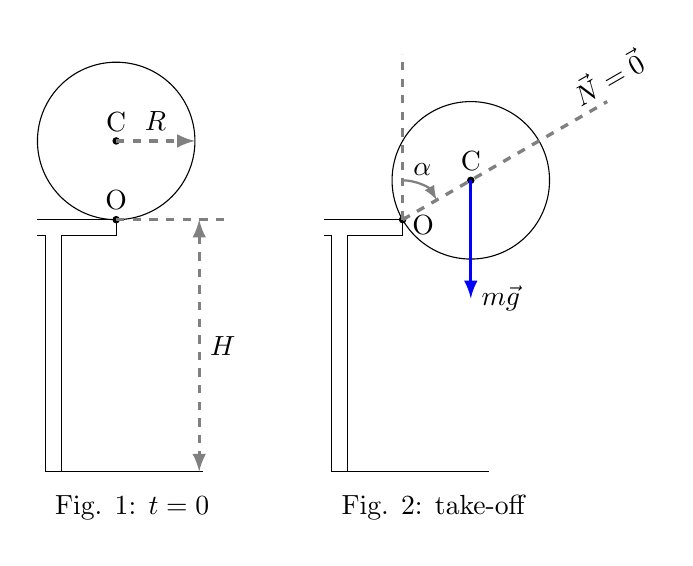
\begin{tikzpicture}[
      force/.style={>=latex,draw=blue,fill=blue, very thick},
      axis/.style={densely dashed,gray,font=\small},
      M/.style={rectangle,draw,fill=lightgray,minimum size=0.5cm,thin},
      m/.style={rectangle,draw=black,fill=lightgray,minimum size=0.3cm,thin},
      plane/.style={draw=black,fill=blue!10},
      string/.style={draw=red, thick},
      pulley/.style={thick},
  ]
  \matrix[column sep=1cm] {
      % Table
      \draw (-1, -1) coordinate (tblleft) -- ++(1,0) coordinate(tblright);
      \draw (tblright) -- ++(0, -0.2) -- ++(-0.7, 0) coordinate(tblbotleft);
      \draw (tblbotleft) -- ++(0, -3) -- ++(-0.2, 0)  coordinate (floorsurfleft);
      \draw (floorsurfleft) -- ++(0, 3) -- ++(-0.1, 0);

      %floor
      \draw (floorsurfleft) -- ++(2, 0) coordinate (floorsurfright);

      \draw[above=1cm of tblright] circle (1cm) coordinate (objcenter);
      \draw[fill=black] (objcenter) circle (0.04cm);
      \node[above = 0em of objcenter.north east]{C};

      %\node[draw=black,fill=black, circle, above = 0em of tblright]{};
      \draw[fill=black] (tblright) circle (0.04cm);
      \node[above = 0em of tblright.north east]{O};

      \draw[>=latex,->,draw=gray,dashed, very thick] (objcenter) -- ++(1cm, 0) node[midway, above]{$R$};
      \draw[>=latex,<->, draw=gray,dashed,very thick] ([xshift=3em]tblright.east) -- ++(0, -3.2) node[midway, right]{$H$};

      \draw[draw=gray,dashed, very thick] (tblright) -- ++(4em, 0);
      \node[below = 0.5em of floorsurfleft.south, anchor=north west]{Fig. 1: $t=0$};
  &
      %%%

      % Table
      {
      \draw (2, -1) coordinate (tblleft) -- ++(1,0) coordinate(tblright);
      \draw (tblright) -- ++(0, -0.2) -- ++(-0.7, 0) coordinate(tblbotleft);
      \draw (tblbotleft) -- ++(0, -3) -- ++(-0.2, 0)  coordinate (floorsurfleft);
      \draw (floorsurfleft) -- ++(0, 3) -- ++(-0.1, 0);

      %floor
      \draw (floorsurfleft) -- ++(2, 0) coordinate (floorsurfright);

      \draw ([xshift=0.866cm,yshift=0.5cm]tblright) circle (1cm) coordinate (objcenter);
      \draw[fill=black] (objcenter) circle (0.04cm);
      \node[above = 0em of objcenter.north east]{C};

      %\node[draw=black,fill=black, circle, above = 0em of tblright]{};
      \draw[fill=black] (tblright) circle (0.04cm)  coordinate (pointO);
      \node[below right = -0.5em and 0em of tblright.east]{O};

      \draw[draw=gray,dashed, very thick] (tblright) -- ++(0, 6em);
      \draw[draw=gray,dashed, very thick] (tblright) -- ++(2.598cm, 1.5cm) node[above=-0.6em]{\rotatebox{30}{$\vec{N} = \vec{0}$}};

      % angle alpha
      \draw[draw=gray, thick,->,>=latex] ([yshift=0.5cm] pointO) arc (90:30:0.5cm) node[midway, above]{$\alpha$};

      % Forces
      \draw[->,force] (objcenter) -- ++(0, -1.5cm) node[right]{$m\vec{g}$};

      \node[below = 0.5em of floorsurfleft.south, anchor=north west]{Fig. 2: take-off};
      }

  \\
  };
  \end{tikzpicture}
  \caption{Do not forget!
  Make it explicit enough that readers
  can figure out what you are doing.}
  \end{figure}
\end{document}
